\documentclass[11pt]{article}

\usepackage{sectsty}
\usepackage{graphicx}

% Margins
\topmargin=-0.45in
\evensidemargin=0in
\oddsidemargin=0in
\textwidth=6.5in
\textheight=9.0in
\headsep=0.25in

% Images
\graphicspath{ {./images/} }

\title{RWTH Aachen University - LELY Challenge Documentation}
\author{RWTH Team}
\date{\today}

\begin{document}
	\maketitle	
	
	\section{Robot A}
	
	\subsection{Overview}
	Robot A is a LIDAR-capable platform. Due to the walls of the challenge being only 37cm talls, the mounting point of the LIDAR is on the bottom front of the chasis, providing a 200 degree field of view.
	
	PICTURE OF COMPLETE ROBOT
	
	\subsection{Sensors}
	A RPLIDAR A1M8-R6 LIDAR is mounted on the front of the robot. The LIDAR interfaces with the laptop directly over USB. 
	
	OFFICIAL PICTURE OF LIDAR
	
	\subsection{Hardware}
	A 3D-printed mount was created for easy placement and adjustment of the LIDAR.
	
	\begin{figure}[h]
		\centering
		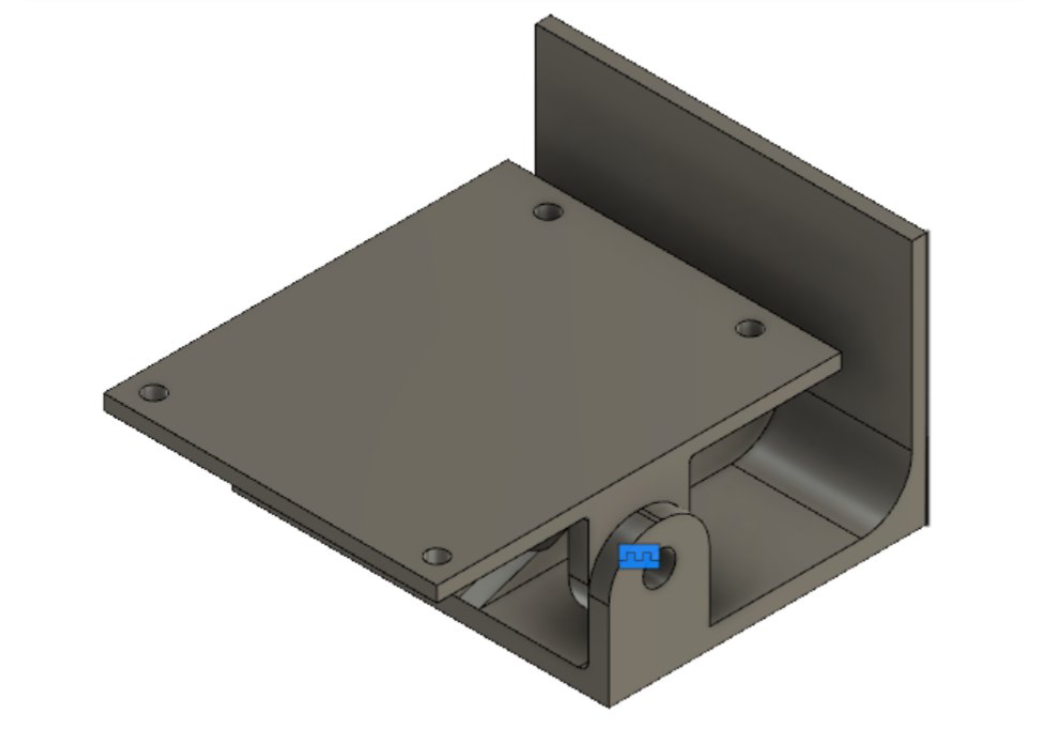
\includegraphics[scale=0.6]{lidar_mount}
		\caption{CAD rendering of LIDAR mount}
	\end{figure}
	
	\subsection{Software}	
	Robot A implements a wall following algorithem. Five equally-spaced lines in front of the robot are sampled via LIDAR.
	
	\pagebreak

	\section{Robot B}
	
	
	\subsection{Overview}
	Robot B uses ultrasonic sensors mounted via aluminium frame to navigate its environment.
	
	PICTURE OF COMPLETE ROBOT
	
	\subsection{Sensors}
	Three HC-SR04 ultrasonic sensors are placed ??somewhere?? around the robot. The sensors interface with the laptop via an Arduino Uno.
	
	OFFICIAL PICTURES OF SENSOR AND ARDUINO.
	
	\subsection{Hardware}
	An aluminium frame with 3D-printed connection points extends from the top mounting point to the bottom of the robot, allowing the sensors to attach to a low-enough point to read the walls of the maze.
	
	PICTURE OF FRAME.
	
	\begin{figure}[h]
		\centering
		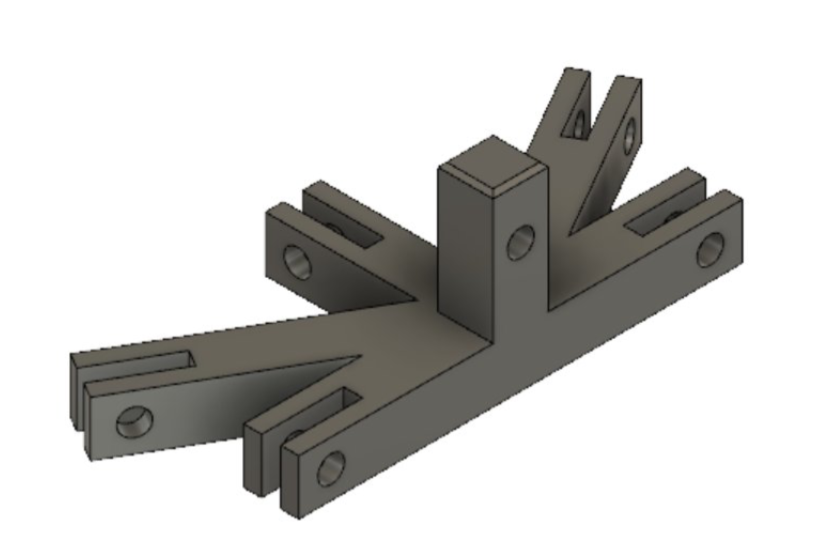
\includegraphics[scale=0.5]{central_mount_empty}
		\caption{Central mount for connection points}
	\end{figure}

	\begin{figure}[h]
		\centering
		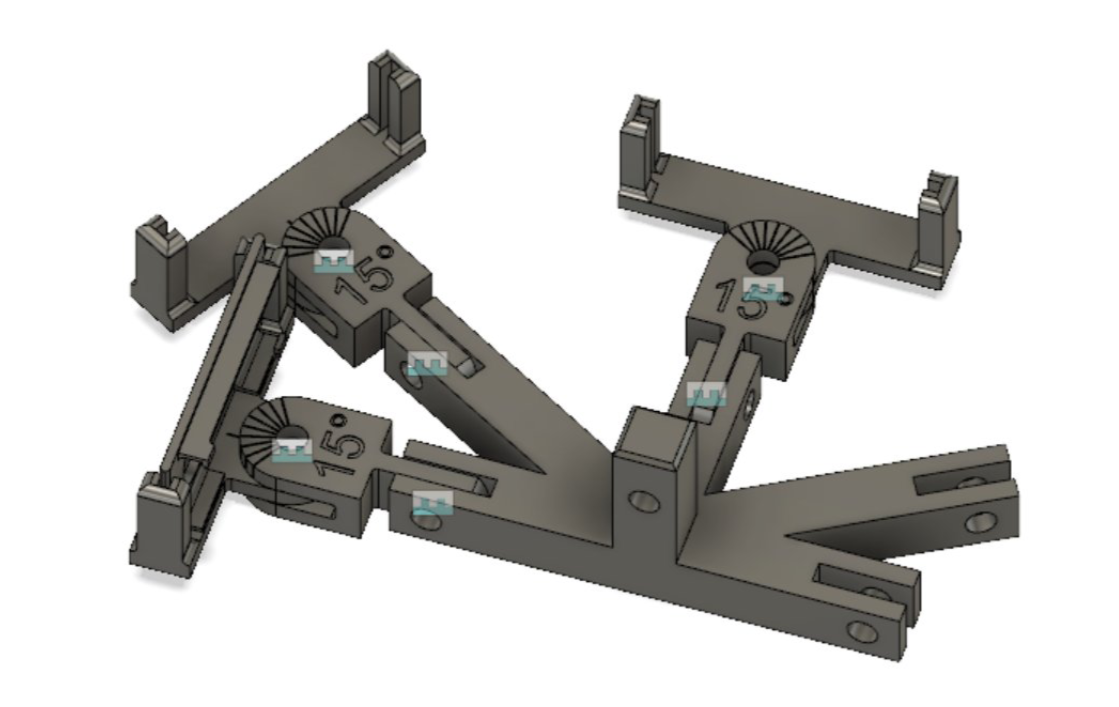
\includegraphics[scale=0.5]{central_mount_conns}
		\caption{Central mount with connections for ultrasonic sensors}
	\end{figure}

	\pagebreak
	
	\subsection{Software}
	DESCRIPTION OF SOFTWARE
	
\end{document}